\documentclass[11pt]{article}
\usepackage[english,serbian]{babel}
\usepackage{graphicx}
\usepackage{epsfig}
\begin{document}
\section{Uvod}

    Zvuk je vibracija koja se širi kroz vazduh (ili neku drugu sredinu) u vidu talasa. Čovek može čuje zvuk jačine od 16 do 20000 Hz (kao što se vidi na slici 1). Ispod ove granice je \textit{infrazvuk}, a iznad \textit{ultrazvuk}. Osnovne karakteristike zvuka su visina, boja i jačina.
    \begin {itemize}
        \item[-] \textit{Visina zvuka} određena je njegovom osnovnom frekvencijom (više tonove stvaraju talasi
        veće frekvencije i obrnuto).
    
        \item[-] \textit{Boja zvuka} je određena karakterom oscilovanja zvučnih talasa. Obično, zvuk nije prost
        harmonijski talas, već je složen iz viših harmonika. Složenost talasa, broj i spektar viših
        harmonika određuje boju zvuka. Parni harmonici daju zvuku toplinu i mekoću, a neparni
        oštrinu i hladnoću.
    
        \item[-] \textit{Jačina zvuka} (I) određena je količinom energije koju zvučni talas prenese u jedinici
        vremena kroz jediničnu površinu koja je normalna na pravac prostiranja talasa. Izražava se
        u vatima po kvadratnom metru.
    \end{itemize}
 
    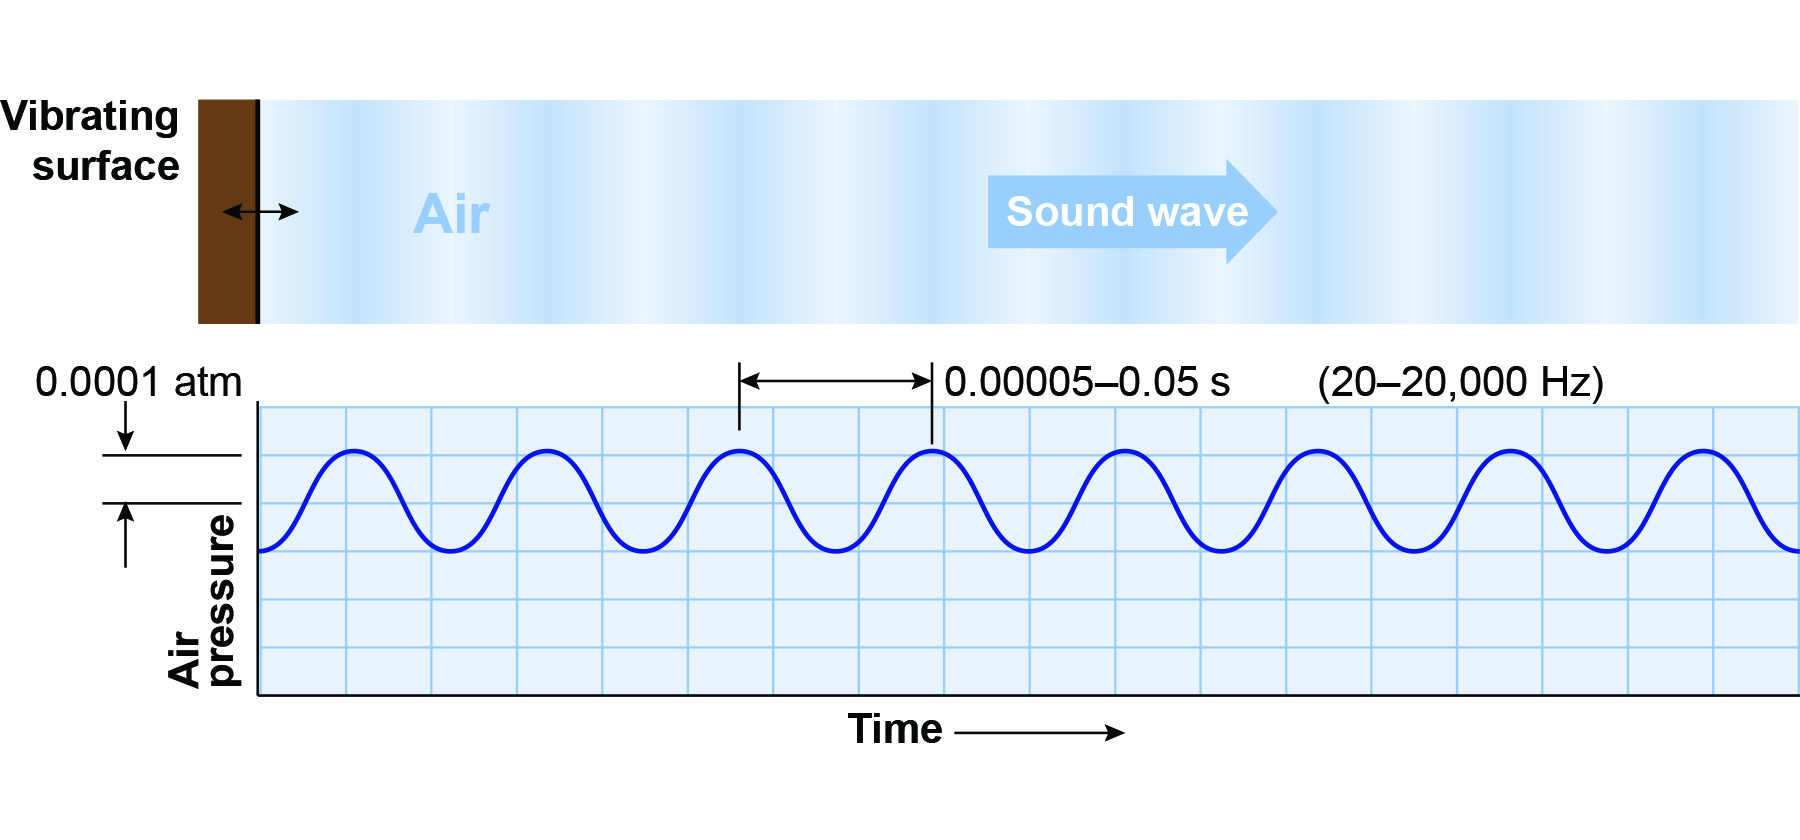
\includegraphics[width=0.8\textwidth]{airpressure}
  \begin{center}
  slika 1
  \end{center}
    \section{Počeci snimanja zvuka}
    \subsection {Analogni zapis zvuka}
    U početku je snimanje zvuka bilo analogno, odnosno, zapisivale su se vibracije koje ljudsko uho prepoznaje kao zvuk na neku vrstu medija. 
    Prvi zvuk je snimljen uz pomoć fonoautografa sredinom 19. veka. Zatim, Emile Berliner je 1889. godine osmislio gramofon koji je mogao da reprodukuje zvuk gotovo 4 minuta. Edison je 1927. patentirao ploču
    koja je mogla da snima 40 minuta zvučnog zapisa, ali se nije proslavio njom. Godine 1928. Fritz Pfleumer je izumeo magnetnu traku i ovaj način snimanja se koristio za vreme Drugog svetskog rata.Nakon toga se pojavila
    stereo magnetna traka koja se mogla koristiti u kućnoj upotrebi. Kompaktna traka i uređaj koji snima i reprodukuje zvuk sa kasete su se pojavili 1964. godine.Kompanija Sony je krajem 80-ih godina predstavila
    novi proizvod DAT (engl.\textit {digital audio tape} ).Ovaj proizvod je prihvaćen od strane raznih industrija jer je mnogo manji od svih prethodnih.
    \subsection {Digitalni zapis zvuka}
    Prvi pokušaj da se kompjuterske obrade zvuka koji je doveo do uspešne digitalne
    transformacije zvuka desio se početkom 1969. godine u Bel Laboratoriji (\textit {Bell
    Labs}), gde je uspešno proizveden veštački, kompjuterski generisan zvuk. U to vreme su se proizvodili PCM procesori. Oni su pretvarali zvuk u digitalni zapis, pa je napravljen eksperimentalni laserski disk. Zatim, početkom 80-ih, pojavljuju se kompaktni diskovi nepristupačne cene, što se ubrzo menja. Patentirani su kompaktni diskovi (CD-RW) koji imaju mogućnost pisanja i brisanja podataka. Napokon, javlja se uređaj koji može da reprodukuje zapisani zvučni zapis - MP3.

\end{document}